\subsection{Speichern \& Export}

Nachdem eine Berechnung in der \gls{bts} erfolgreich durchgef�hrt wurde und die Performancedaten angezeigt werden, gibt es zwei M�glichkeiten diese zu sichern: das Speichern und das Exportieren. \\
\\
Beim Speichern werden alle Einstellungen des Settings-Tab sowie alle allgemeinen und Order-spezifischen Performancedaten bin�r serialisiert (Siehe \ref{Binaere-Serialisierung} ''Bin�re Serialisierung'') und in ein spezielles .bts-File gespeichert. Dieses kann zu einem sp�teren Zeitpunkt auch wieder geladen werden, wobei der komplette Zustand der \gls{bts} bis auf das gezeichnete Chart wiederhergestellt wird. Dies funktioniert vor allem recht einfach, da bei jedem Speicher- sowie Lese-Vorgang die serialisierten Daten in der selben Reihenfolge gespeichert bzw. ausgelesen werden k�nnen. Wie die \gls{bts} nach dem Laden ohne Chart aussieht, kann der Abbildung \ref{fig:bts_order_geladen} entnommen werden.\\

\begin{figure}[!h]
	\centering
		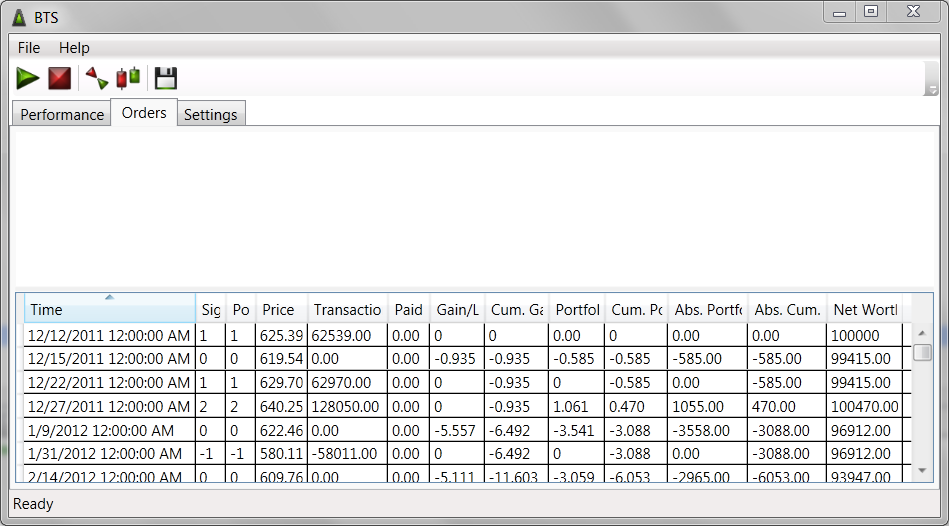
\includegraphics[width=0.90\textwidth]{graphics/ergebnis/bts_order_geladen.png}
	\caption{Beispielhafte Darstellung des Orders-Tab nach Laden eines .bts-Files}
	\label{fig:bts_order_geladen}
\end{figure}

Das Exportieren ist das f�r Menschen lesbare Gegenst�ck zum Speichern. Hier wird ein einfaches .txt-File mit allen allgemeinen Performancedaten exportiert, damit diese bspw. zum Vergleich verschiedener Algorithmen herangezogen werden k�nnen. Ein auf diese Art und Weise exportiertes File sieht in etwa aus wie der folgende Code:

\begin{verbatim}
Algorithm used: multipleRegressions.dll
Data-File used: GOOG_1dBar_20130110.csv

Net Worth:                                     130033,600
											  (+30033,600)
Portfolio Performance [%]:                     30,034
Sharpe Ratio:                                  9,996
Mean Deviation of Portfolio Performance [%]:   2,824
Mean Deviation of Equity Price:                51,993
Return on Investment [%]:                      38,384
Number of Good Trades:                         15
Gain From Good Trades [%]:                     43,213
Number of Bad Trades:                          7
Loss From Bad Trades [%]:                     -13,179
Ratio of Good Trades - Bad Trades:             2,143
\end{verbatim}

Sowohl das Speichern und Laden als auch das exportieren benutzen speziellen FileDialogs (\textit{OpenFileDialog} und \textit{SaveFileDialog}) zur Auswahl der zu ladenden Datei bzw. dem gew�nschten Speicherort der Datei. Diese FileDialog sieht bspw. beim Speichern eines .bts-Files aus wie in Abbildung \ref{fig:bts_speichern}.\\

\begin{figure}[!h]
	\centering
		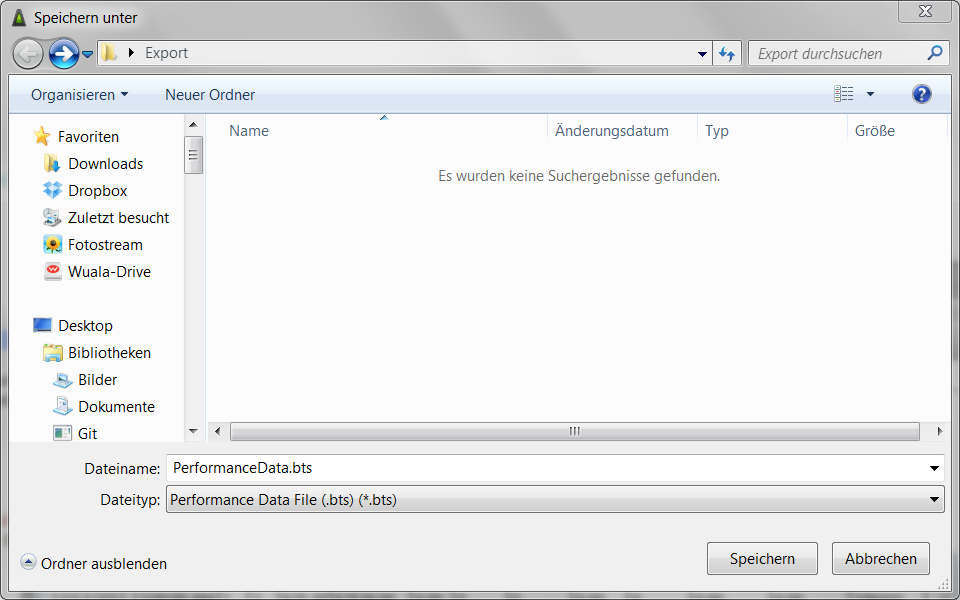
\includegraphics[width=0.90\textwidth]{graphics/ergebnis/bts_speichern.png}
	\caption{\textit{SaveFileDialog} beim Speichern eines .bts-Files}
	\label{fig:bts_speichern}
\end{figure}

Nach dem Speichern/Exportieren befinden sich die Dateien dann auch wirklich im angegebenen Ordner, wie man in Abbildung \ref{fig:bts_settings_export} erkennen kann.

\begin{figure}[!h]
	\centering
		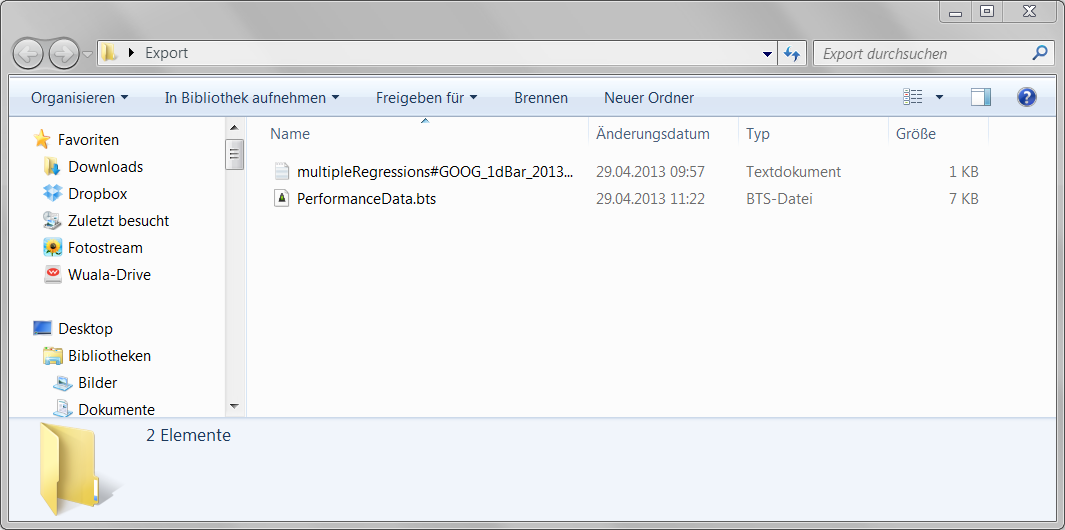
\includegraphics[width=0.90\textwidth]{graphics/ergebnis/bts_settings_export.png}
	\caption{Ordner mit einem gespeicherten Zustand und einem Export der BTS}
	\label{fig:bts_settings_export}
\end{figure}